\documentclass[8pt]{beamer}
\usetheme{default} % Very simple theme
\usecolortheme{dove} % Minimalist grayscale colors
\setbeamertemplate{navigation symbols}{} % Remove navigation bar

% Define brand-like colors
\definecolor{myblue}{RGB}{0, 102, 204}    % Blue for standard blocks
\definecolor{mygreen}{RGB}{0, 153, 0}     % Green for example blocks
\definecolor{myred}{RGB}{204, 0, 0}       % Red for alert blocks
\definecolor{myorange}{RGB}{255, 128, 0} % For \emph

% Accent color for titles, bullets, etc.
\setbeamercolor{structure}{fg=myblue}

% Block colors
\setbeamercolor{block title}{bg=myblue, fg=white}
\setbeamercolor{block body}{bg=blue!5, fg=black}

\setbeamercolor{exampleblock title}{bg=mygreen, fg=white}
\setbeamercolor{exampleblock body}{bg=green!5, fg=black}

\setbeamercolor{alertblock title}{bg=myred, fg=white}
\setbeamercolor{alertblock body}{bg=red!5, fg=black}
\setbeamercolor{alerted text}{fg=myred}

% Optional: color for \example text
\setbeamercolor{example text}{fg=mygreen}

% Custom emph (orange text instead of italic)
\let\oldemph\emph
\renewcommand{\emph}[1]{\textcolor{myorange}{#1}}
\newcommand{\ve}[1]{\boldsymbol{#1}}

\usepackage{graphicx} % Package for images
\usepackage{amsmath} % Package for images
\graphicspath{{figs/}} % Path to your figures directory
\usepackage{array}  % For better column spacing
\usepackage{caption} % Required for \captionof
\usepackage{tikz}
\usetikzlibrary{calc,positioning,arrows.meta,shapes.geometric}
%\usepackage{enumitem}

% Title Information
\title{STOCHASTIC METHODS IN WATER RESOURCES}
\vspace{25pt}
\subtitle{Unit 6: Stochastic modelling and prediction \\ Lecture 19: Stochastic Differential Equations in Hydrology}
\author{Luis Alejandro Morales, Ph.D.}
\institute{Universidad Nacional de Colombia \\ Department of Civil and Agriculture Engineering} %// }
%\date{\today}

\begin{document}

% Title Slide
\begin{frame}
    \titlepage
\end{frame}

%------------------------------------------------
\begin{frame}{Motivation in Hydrology}
Hydrological systems are subject to:
\begin{itemize}
 \item Random rainfall variability
 \item Subsurface heterogeneity
 \item Measurement noise and model uncertainty
\end{itemize}

Deterministic ODEs fail to represent these effects.\\
\textbf{SDEs explicitly incorporate randomness:}
\[
 dX_t = f(X_t,t)\,dt + g(X_t,t)\,dW_t
\]
where $W_t$ is a Wiener process.\\
A \textbf{Wiener Process (Brownian Motion)} $W(t)$ is a stochastic process defined by:

\begin{itemize}
    \item $W(0) = 0$
    \item Continuous paths: $W(t)$ is almost surely continuous.
    \item Independent increments: $W(t) - W(s)$ independent of past for $t > s$.
    \item Gaussian increments:
    \[
    W(t) - W(s) \sim \mathcal{N}(0,\, t-s)
    \]
\end{itemize}
\end{frame}

% \begin{frame}{Mean Evolution in Stochastic Hydrological Systems}

% \textbf{Definition (Hydrological Interpretation)}

% Let $X(t)$ represent a hydrological state variable, such as:
% \begin{itemize}
    % \item River discharge
    % \item Soil moisture
    % \item Groundwater head
% \end{itemize}

% modeled by a Stochastic Differential Equation (SDE):
% \[
% dX(t) = f(X,t)\,dt + g(X,t)\,dW(t)
% \]
% where $W(t)$ is a Wiener process representing random rainfall, infiltration variability, or climate noise.

% \vspace{0.3cm}

% \textbf{Mean Evolution Property:}
% \[
% \mathbb{E}[X(t)] \neq X_{det}(t)
% \]

% \begin{block}{Meaning}
% The expected (average) hydrological response of the stochastic system does not follow the trajectory predicted by the deterministic model obtained by neglecting randomness.
% \end{block}

% \begin{itemize}
    % \item Noise alters the system dynamics, not just short-term variability.
    % \item Random precipitation and subsurface heterogeneity shift the mean response.
    % \item The deterministic model underestimates or misrepresents long-term behavior.
% \end{itemize}

% \textbf{Implication:}
% Using purely deterministic models can lead to biased predictions of flood peaks, recharge rates, and storage evolution.

% \end{frame}
%------------------------------------------------
\begin{frame}{Deterministic ODE vs Stochastic SDE}
\textbf{Deterministic model}
\[
\frac{dS}{dt} = I(t) - Q(S)
\]
Unique trajectory for given initial condition.

\vspace{0.3cm}
\textbf{Stochastic model}
\[
dS = (I - kS)dt + \sigma dW_t
\]
Produces ensemble of possible trajectories.

\begin{itemize}
 \item ODE: no uncertainty propagation
 \item SDE: state variance evolves in time
\end{itemize}
\end{frame}

%------------------------------------------------
\begin{frame}{General Form of SDE}
Hydrological state variable $X(t)$ (flow, storage, soil moisture):
\[
dX(t) = a(X,t)dt + b(X,t)dW_t
\]

Components:
\begin{itemize}
 \item Drift $a(X,t)$: physical dynamics
 \item Diffusion $b(X,t)$: stochastic forcing
\item $dW(t)$: infinitesimal increment of Wiener process
\end{itemize}

Mean evolution:
\[
\mathbb{E}[X(t)] \neq X_{det}(t)
\]
which means that the average (mean)($\mathbb{E}[.]$ ) behavior of a stochastic system ($X(t)$) is not the same as the solution of the corresponding deterministic system $X_{det}(t)$

\end{frame}

%------------------------------------------------
\begin{frame}{Conceptual Diagram of SDE}
\centering
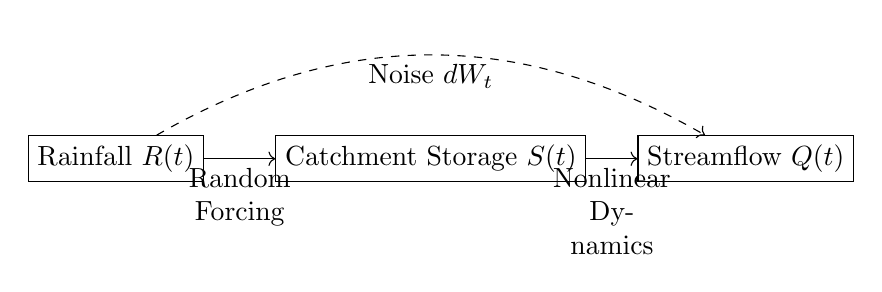
\begin{tikzpicture}[node distance=4cm]
 \node (rain) [draw, rectangle] {Rainfall $R(t)$};
 \node (storage) [draw, rectangle, right of=rain] {Catchment Storage $S(t)$};
 \node (flow) [draw, rectangle, right of=storage] {Streamflow $Q(t)$};

 \draw[->] (rain) -- node[below, align=center, text width=1.5cm]{Random Forcing} (storage);
 \draw[->] (storage) -- node[below, align=center, text width=1.5cm]{Nonlinear Dynamics} (flow);
 \draw[->, dashed] (rain) to[bend left] node[below]{Noise $dW_t$} (flow);
\end{tikzpicture}

Compact conceptualization of stochastic rainfall-runoff.
\end{frame}

%------------------------------------------------
\begin{frame}{It\^o Interpretation}
Increment form:
\[
\Delta X = a(X,t)\Delta t + b(X,t)\Delta W
\]

Properties of Wiener process:
\[
\mathbb{E}[dW_t]=0, \quad Var(dW_t)=dt
\]

Important result:
\[
(dW_t)^2 = dt
\]
This alters chain rule (It\^o lemma).
\end{frame}

\begin{frame}{It\^o Calculus in Rainfall--Runoff and Groundwater Systems}

\textbf{Hydrological Context}

Let $X(t)$ represent a hydrological state variable such as:
\begin{itemize}
    \item River discharge $Q(t)$ (rainfall--runoff)
    \item Groundwater head $h(t)$ (aquifer storage dynamics)
\end{itemize}

These variables are influenced by uncertain forcing:
\begin{itemize}
    \item Random rainfall events
    \item Spatial heterogeneity of soil and aquifer properties
    \item Climate variability
\end{itemize}

\textbf{Stochastic Hydrological Model (It\^o SDE)}
\[
dX(t) = f(X,t)\,dt + g(X,t)\,dW(t)
\]

\vspace{-5pt}
where:
\begin{itemize}
    \item $f(X,t)$ represents deterministic hydrological processes (infiltration, recharge, drainage),
    \item $g(X,t)$ controls the intensity of random forcing,
    \item $W(t)$ is a Wiener process modeling rainfall uncertainty.
\end{itemize}


\textbf{Key It\^o Property}
\[
(dW)^2 = dt
\]

This implies that randomness modifies the physical evolution of the system, introducing an additional drift component.

\textbf{Physical Interpretation}
\begin{itemize}
    \item Random rainfall does not only cause fluctuations — it alters the mean hydrograph.
    \item Groundwater recharge becomes statistically shifted under stochastic forcing.
    \item Flood peaks and storage dynamics deviate from deterministic predictions.
\end{itemize}
\vspace{-1pt}

Ignoring stochastic forcing can lead to biased flood risk estimation and misrepresentation of long-term groundwater behavior.

\end{frame}

%------------------------------------------------
\begin{frame}{Euler--Maruyama Scheme}
Numerical integration for SDE:
\[
X_{n+1} = X_n + a(X_n,t_n)\Delta t + b(X_n,t_n)\sqrt{\Delta t}\,Z_n
\]
where:
\begin{itemize}
 \item $Z_n \sim \mathcal{N}(0,1)$
 \item Monte Carlo simulation produces ensemble
\end{itemize}

Used in:
\begin{itemize}
 \item Flood routing uncertainty
 \item Basin storage estimation
\end{itemize}
\end{frame}

%------------------------------------------------
\begin{frame}{Example: Stochastic Linear Reservoir}
Model storage $S(t)$:
\[
dS = (R - kS)dt + \sigma dW_t
\]
\begin{itemize}
    \item $S(t)$ : Water storage at time $t$  
    (soil moisture, reservoir storage, or groundwater storage)

    \item $dS$ : Infinitesimal change in storage over time interval $dt$

    \item $R$ : Mean recharge or effective rainfall input  
    (average inflow to the system)

    \item $k$ : Recession or drainage coefficient  
    (controls how fast water leaves the system)

    \item $kS$ : Storage-dependent outflow  
    (baseflow, percolation, evapotranspiration losses)

    \item $\sigma$ : Noise intensity  
    (magnitude of rainfall or recharge variability)

    \item $W_t$ : Wiener process (Brownian motion)  
    representing random rainfall or climate fluctuations

    \item $dW_t$ : Random perturbation applied to storage
\end{itemize}
Discretized:
\[
S_{n+1} = S_n + (R - kS_n)\Delta t + \sigma \sqrt{\Delta t} Z_n
\]
Streamflow:
\[
Q_n = k S_n
\]

Represents rainfall-runoff with noise.
\end{frame}

%------------------------------------------------
\begin{frame}{Worked Numerical Example}
Let:
\begin{itemize}
 \item $R=10$ mm/h
 \item $k=0.2$ h$^{-1}$
 \item $\sigma=1.5$
 \item $\Delta t=1$ h, $S_0=20$
 \item $Z_0=0.4$
\end{itemize}

Step 1:
\[
S_1 = 20 + (10 - 0.2\times20)(1) + 1.5(1)(0.4)
\]
\[
S_1 = 20 + (10 - 4) + 0.6 = 26.6
\]
Then $Q_1 = 0.2 \times 26.6 = 5.32$ mm/h
\end{frame}

%------------------------------------------------
\begin{frame}{Hydrological Applications}
\begin{itemize}
 \item Flood wave propagation with uncertainty
 \item Groundwater head fluctuation modeling
 \item Soil moisture stochastic balance
 \item Climate-driven runoff variability
 \item Real-time forecasting with noise-aware models
\end{itemize}

SDEs provide physically realistic uncertainty dynamics.
\end{frame}

%------------------------------------------------
\begin{frame}{Advantages and Limitations}
\textbf{Advantages}
\begin{itemize}
 \item Explicit uncertainty representation
 \item Realistic ensemble generation
 \item Suitable for data assimilation
\end{itemize}

\textbf{Limitations}
\begin{itemize}
 \item Requires stochastic calculus
 \item Parameter estimation more complex
 \item Computationally intensive
\end{itemize}
\end{frame}

%------------------------------------------------
\begin{frame}{Summary}
\begin{itemize}
 \item SDEs extend hydrological models by including randomness
 \item Governed by drift + diffusion components
 \item Solved numerically with Euler--Maruyama
 \item Useful for realistic flood and runoff modeling
 \item Foundation for Kalman filtering and data assimilation
\end{itemize}

\centering
\textbf{SDEs bridge physics and uncertainty in modern hydrology.}
\end{frame}

\end{document}
